\usetikzlibrary{calc,arrows.meta,positioning,backgrounds}
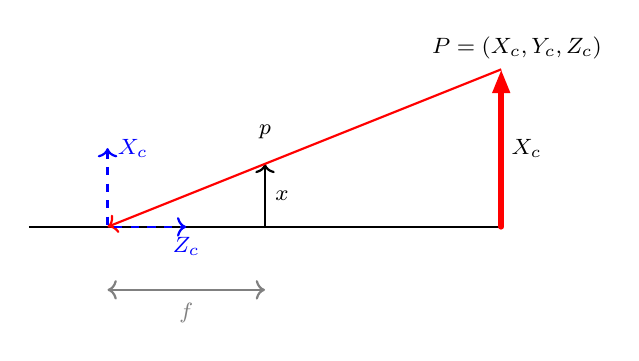
\begin{tikzpicture} [
    description/.style={draw=gray!70, thick, line cap=round, every node/.style={align=center, font=\scriptsize\sffamily, anchor=north}},
imagearrow/.style={red, line cap=round, -{Triangle[width=3*#1]}, line width=#1, shorten >=#1*0*1.75pt, every node/.append style={fill, circle, inner sep=0pt, minimum size=#1*3.5pt, anchor=center, outer sep=0pt}}
  ]

\tikzstyle{every node}=[font=\footnotesize]

\draw[thick] (-1,0) -- (5,0);

 \draw [->,thick] (2,0) -- (2,0.8) ;
\draw [thick](2,0.4) node[right]{$x$};
\draw [thick](2,1.2) node{$p$};

 %\draw [thick, red] (5,0) -- (5,2);
 \draw [imagearrow = 2] (5,0) -- (5,2);

\draw [thick](5,1) node[right]{$X_c$};
\draw [thick](5.2,2) node[above]{$P=(X_c,Y_c,Z_c)$};

\draw[->,red, thick] (5,2) -- (0,0);

\draw[gray, <->, thick] (0,-0.8) -- (2,-0.8);
\draw[gray] (1,-1.1) node{$f$};

% coordinate systems
\draw [<->,thick, blue, dashed] (0,1) node (yaxis) [right] {$X_c$}
        |- (1,0) node (xaxis) [below] {$Z_c$};

\end{tikzpicture}